\documentclass[aps,prd,twocolumn,superscriptaddress,preprintnumbers,floatfix,nofootinbib]{revtex4-2}

\usepackage{showyourwork}
\usepackage{amsfonts,amssymb,amsmath}

\begin{document}

\title{Constraining gravitational wave amplitude birefringence with GWTC-3}

\author{Thomas C. K. Ng}
\email{thomas.ng@link.cuhk.edu.hk}
\affiliation{Department of Physics, The Chinese University of Hong Kong, Shatin, Hong Kong}

\author{Maximiliano Isi}
\email{misi@flatironinstitute.org}
\affiliation{Center for Computational Astrophysics, Flatiron Institute, 162 5th Ave, New York, NY 10010, United States}

\author{Kaze W. K. Wong}
\email{kwong@flatironinstitute.org}
\affiliation{Center for Computational Astrophysics, Flatiron Institute, 162 5th Ave, New York, NY 10010, United States}

\author{Will M. Farr}
\email{wfarr@flatironinstitute.org}
\affiliation{Center for Computational Astrophysics, Flatiron Institute, 162 5th Ave, New York, NY 10010, United States}
\affiliation{Department of Physics and Astronomy, Stony Brook University, Stony Brook NY 11794, United States}

\date{\today}

\begin{abstract}
    One of the major problems physicists face nowadays is that Einstein's theory of general relativity (GR) does not agree with quantum theories at some length scales.
    In recent decades, theorists have worked on many beyond-GR theories to unify both.
    Some of these theories, such as Chern-Simons gravity, suggest that there is gravitational wave (GW) amplitude birefringence.
    In our study, we perform parameter estimation (PE) to constrain the strength of GW amplitude birefringence.
    Compared to previous studies, we performed PE on more events, including events in the third LIGO-Virgo catalog (GWTC-3), and used a more realistic birefringence model to describe the phenomenon.
    We obtained a constraint tighter than previous studies for an order of magnitude.
\end{abstract}

\maketitle

\section{Introduction}
\label{sec:Introduction}
% Motivation
Gravitational waves (GWs) have been used to test Einstein's theory of general relativity (GR) with detections by LIGO-Virgo-KAGRA Collaboration (LVK) \citep{LIGO, Virgo, KAGRA}.
To study the possibility of different beyond-GR theories, we can observe if GWs have any deviation from GR.
Some beyond-GR theories, such as Chern-Simons gravity, suggest that there is gravitational wave amplitude birefringence, while GR predicts no birefringence.
GW amplitude birefringence is a property of space-time that consists of the enhancement of one GW polarization over the other as the wave propagates.

% Previous studies
Previous studies have constrained amplitude birefringence by performing different statistical analyses.
\citet{Yamada_2020} and \citet{Wang_2021} both performed parameter estimation (PE) on the events in the first GW transient catalog \citep{GWTC-1}, GWTC-1, using birefringence templates.
\citet{Okounkova_2022} considered the distribution of observed inclinations of the GW events in the second GW transient catalog \citep{GWTC-2}, GWTC-2, to look for signs of birefringence.

% What's new?
In this study, we used a frequency-dependent birefringence model to constrain the strength of GW amplitude birefringence by performing PE.
This model is a better approximation of the birefringence effect than the frequency-independent model used in \citet{Okounkova_2022}.
Compared to previous studies, we also performed PE on more events, including events in the third GW transient catalog \citep{GWTC-3}, GWTC-3.
We consider 70 binary black hole merger events with a false alarm rate $\leq1\mathrm{yr^{-1}}$.
These events are also listed in TABLE I in \citet{GWTC-3_population}.\footnote{
GW190720 is included in the list in \citet{GWTC-3_population}, but we did not include it in this study.
Details in Sec.~\ref{sec:GW190720}.}
We then give the population constraint on the strength of GW amplitude birefringence by using the PE results.

% Section guide
In Sec.~\ref{sec:Method}, we describe the modification we made to the waveform model, mention the configuration we used in the PE and show the method we used to obtain the population constraint on GW amplitude birefringence.
In Sec.~\ref{sec:Results}, we present the population constraint on GW amplitude birefringence we obtained and show the results of individual PE.
In Sec.~\ref{sec:Discussion}, we discuss the limitation of this study and provide suggestions for future studies.

\section{Method}
\label{sec:Method}

\subsection{Waveform modification}
% GW polarization
GWs comprise two independent polarization modes, just like electromagnetic waves, which are usually represented in the linear states (i.e. $+$ and $\times$).
For a given Fourier mode, they can be combined into left and right circular states (i.e. left-handed and right-handed).
They are related by
\begin{equation}
    h_{\mathrm{L/R}} = \frac{h_+ \pm i h_\times}{\sqrt{2}}\,,
\end{equation}
where $h_{\mathrm{L/R}}$ are the amplitude of the left-handed and right-handed polarization of the waveform, $h_+$ and $h_\times$ are the amplitude of the plus and cross polarization of the waveform.

% Waveform modification
GW amplitude birefringence would enhance one polarization mode over the other.
In theories like Chern- Simons gravity, the observed Fourier waveform takes the form of
\begin{equation}
    h_\mathrm{L/R}^{\mathrm{br}}=
    h_\mathrm{L/R}^{\mathrm{GR}}\times
    \exp\left(\pm\kappa\frac{d_C}{1\mathrm{Gpc}}\frac{f}{100\mathrm{Hz}}\right)\,,
    \label{eq:waveform_modification}
\end{equation}
where $h_\mathrm{L/R}^{\mathrm{br}}$ is the Fourier amplitude of the observed waveform with amplitude birefringence, $h_\mathrm{L/R}^{\mathrm{GR}}$ is the Fourier amplitude of the waveform emitted, $\kappa$ is the dimensionless opacity parameter that represents the strength of the birefringence, $d_C$ is the comoving distance to the source, and $f$ is the frequency of the waveform.
We assume the intrinsic modification is small, so we can use GR waveform templates to describe the emitted waveform.

Although the intrinsic modification is small, the effect accumulates as the GW propagates.
As the GWs propagate, the effect of birefringence will be built up with the number of cycles which depends on the distance traveled and the frequency of the GWs.
According to equation \ref{eq:waveform_modification}, a positive $\kappa$ means the left-handed polarization is enhanced over the right-handed polarization, while a negative $\kappa$ means the opposite.
Note that when $\kappa=0$, the waveform is the same as GR predicts.

\subsection{Effect on inclination}
% Effect on inclination PE results
In GR, the amplitude ratio of the left-handed and right-handed polarizations only depends on the inclination for the dominant $(2,\pm 2)$ angular mode of nonprecessing binaries.
The relationship between the amplitude ratio and the inclination is
\begin{equation}
    \frac{h_\mathrm{L}}{h_\mathrm{R}}=\left(\frac{1-\cos\iota}{1+\cos\iota}\right)^2\,,
\end{equation}
where $\iota$ is the inclination, the angle between our line of sight and the orbital angular momentum of the binary.
Birefringence can alter the ratio between polarizations of the waveform.
Thus, the birefringence effect could affect the PE result on $\iota$ based on \citet{Okounkova_2022}.

Based on the modification we implemented, the amplitude ratio of the left-handed and right-handed polarizations would be given by
\begin{equation}
    \frac{h_\mathrm{L_{obs}}}{h_\mathrm{R_{obs}}}=\frac{\left(1-\cos\iota\right)^2}{\left(1+\cos\iota\right)^2}\exp\left({2\kappa\frac{d_C}{1\mathrm{Gpc}}\frac{f}{100\mathrm{Hz}}}\right)\,,
    \label{eq:modified_amplitude_ratio}
\end{equation}
where $h_\mathrm{L_{obs}}$ and $h_\mathrm{R_{obs}}$ are the observed amplitude of left-handed and right-handed polarizations of the GWs.
As the amplitude ratio does not only depends on $\iota$ with this modification but also $\kappa$ and $d_C$, the PE results on $\iota$ and $d_C$ are affected.

\citet{Okounkova_2022} assume the effect of birefringence is independent of the frequency, which is a zeroth-order approximation of the birefringence model in Chern-Simons gravity.
This assumption would create a degeneracy between $\kappa$ and $\iota$, as they can affect the amplitude ratio similarly.
To reconstruct the amplitude ratio from the interferometer data, an $\iota$ representing a more face-off inspiral can pair with a positive $\kappa$, or an $\iota$ representing a more face-on inspiral with a negative $\kappa$.

In contrast, we included the frequency dependence in the equation \ref{eq:modified_amplitude_ratio}, which is a first-order approximation of the birefringence model.
The frequency dependence can break the degeneracy between $\kappa$ and $\iota$, as this would make the effect of the birefringence affect the amplitude ratio differently compared to $\iota$.
To illustrate the frequency dependence of amplitude birefringence, the observed amplitudes of two polarizations of a simulated GW signal are shown in figure \ref{fig:birefringence}.

\begin{figure}[h]
    \script{birefringence.py}
    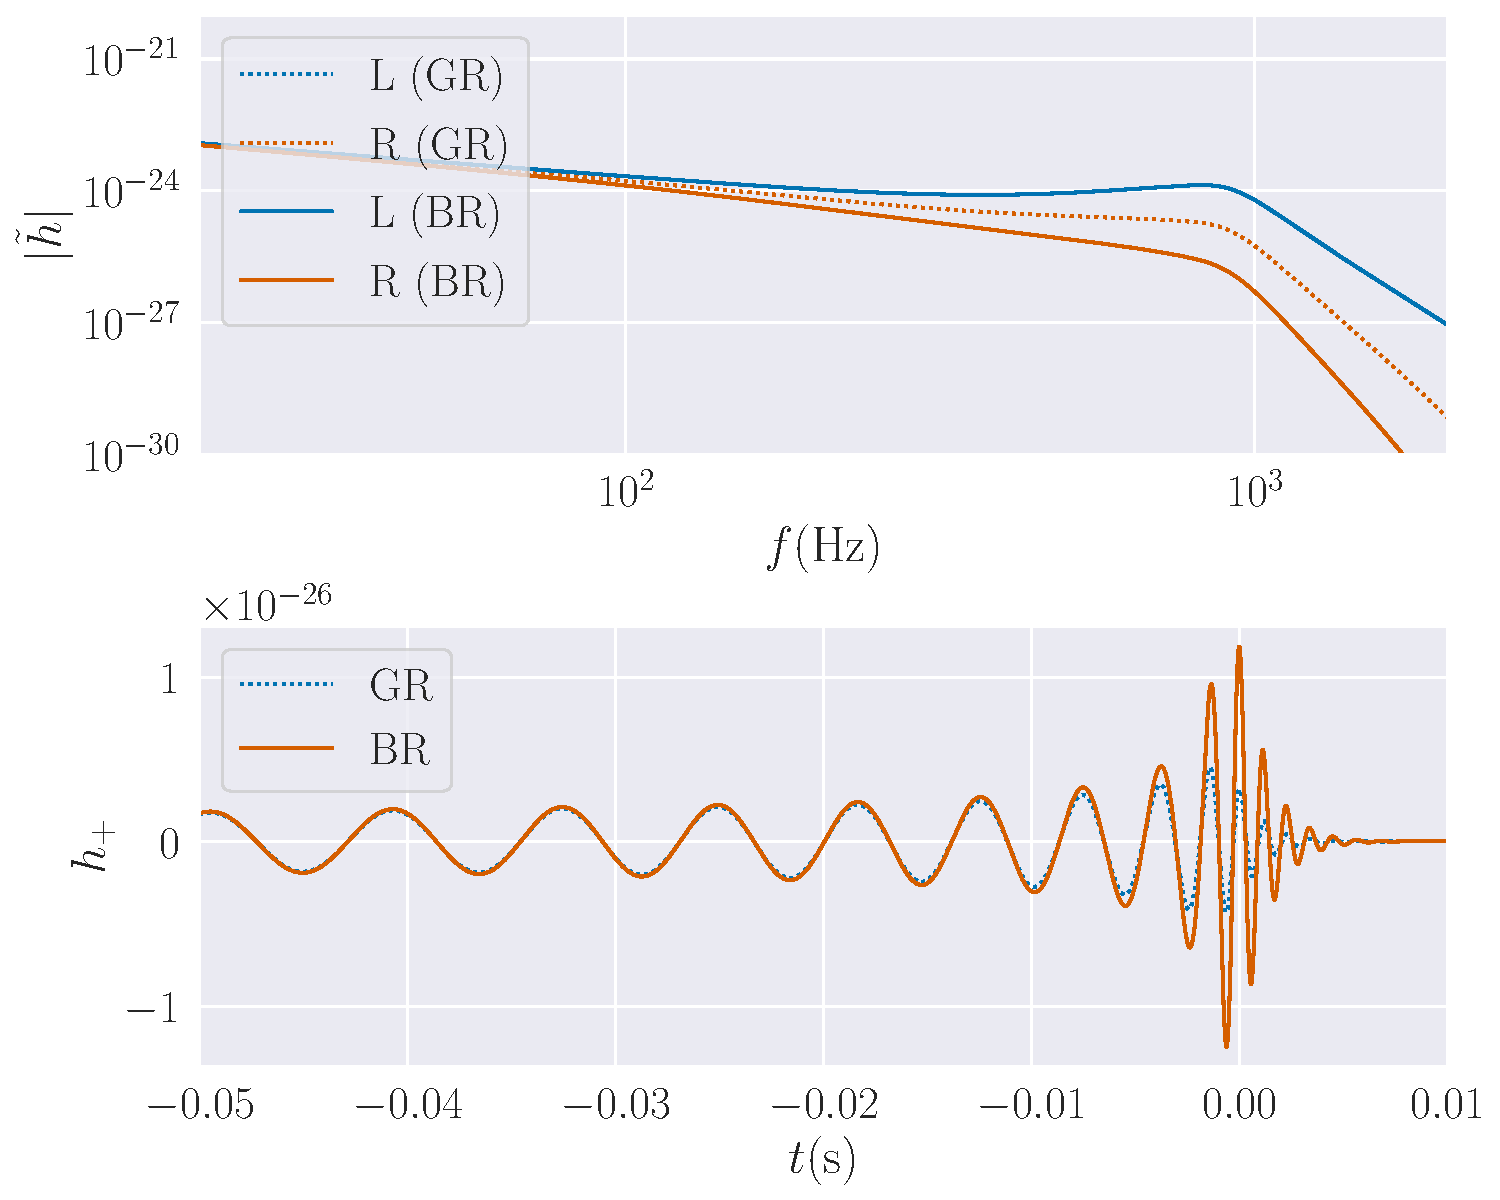
\includegraphics[width=\columnwidth]{figures/birefringence.pdf}
    \caption{
        The observed Fourier amplitude of two polarizations of a simulated GW signal with and without birefringence.
        The amplitudes, as GR predicts, are shown in dotted lines with blue and orange colors representing the left-handed and right-handed polarizations.
        The amplitudes with birefringence are shown in solid lines with blue and orange colors representing the left-handed and right-handed polarizations.
        This plot shows the effect of amplitude birefringence with frequency dependence.
    }
    \label{fig:birefringence}
\end{figure}

\subsection{Parameter estimation}
% Parameter estimation
To constrain $\kappa$, we perform PE with data from the third GW transient catalog \citep{GWTC-2.1, GWTC-3}, GWTC-3, using Bilby \citep{Bilby}, a Bayesian toolkit for GW data analysis which can calculate posteriors of GW parameters based on interferometer data and priors for the parameters in question.
We modified Bilby to include the birefringence effect in the likelihood function.
We then perform PE on intrinsic and extrinsic parameters including $\kappa$ with open data from the Gravitational Wave Open Science Center \citep{GWOSC}.
For PE configuration, we use the same PE configuration as in \citet{GWTC-2.1, GWTC-3} for each event and set the prior on $\kappa$ to a uniform distribution between $-1$ and $1$.
The PE results are published in \citet{dataset}.

We assume $\kappa$ is the same for all events and calculate a posterior distribution of $\kappa$.
The posterior distribution is given by
\begin{equation}
    p(\kappa|\{d\})\propto \prod_{i}p(\kappa|d_i)\,,
    \label{eq:restricted_posterior}
\end{equation}
where $p$ is the probability density function, $i$ is the index of the event, $\{d\}$ is the set of data including all events, and $d_i$ is the data of a single event.
Equation \ref{eq:restricted_posterior} shows that the posterior distribution of $\kappa$ is the product of the posterior distribution of $\kappa$ for each event.
This posterior distribution is a restricted posterior distribution because we assume $\kappa$ is the same for all events.

Note that we also perform a sanity test to check if our PE could recover the PE results done by LVK in \citet{GWTC-2.1, GWTC-3}.
To implement the sanity check, we set $\kappa$ to be $0$, which forces the PE results to be consistent with GR.
These sanity test results are also attached in \citet{dataset}.

\subsection{Bayesian hierarchical modeling}
% Bayesian Hierarchical Modeling

We then perform Bayesian hierarchical modeling to further analyze the constraint on $\kappa$.
Bayesian hierarchical modeling is a method to check if our waveform model can fully describe the amplitude birefringence effect.
Here, instead of assuming all events share the same value of $\kappa$, we assume $\kappa$ from each event is a true value drawn from a Gaussian distribution with mean $\mu$ and standard deviation $\sigma$.
We chose a Gaussian distribution as the underlying distribution of $\kappa$ because it captures the correct mean and the standard deviation of the distribution no matter what the underlying distribution is.

With the posterior of $\kappa$ from PE on each event, the posterior of $\mu$ and $\sigma$ can be calculated by
\begin{equation}
    p(\mu,\sigma|\{d\})\propto p(\mu,\sigma)\prod_{i}\int\frac{p(\kappa_i|d_i)}{p(\kappa_i}p(\kappa_i|\mu,\sigma)\,d\kappa_i\,,
    \label{eq:posterior_of_mu_sigma}
\end{equation}
Note that $p(\kappa)$ is the prior of $\kappa$, which is a uniform distribution between $-1$ and $1$ in this study.
We chose the prior of $\mu$ and $\sigma$ being uniform distributions.
Equation \ref{eq:posterior_of_mu_sigma} can then be simplified to
\begin{equation}
    p(\mu,\sigma|\{d\})\propto\prod_{i}\int p(\kappa_i|d_i)\mathcal{N}(\mu,\sigma)\,d\kappa_i\,.
\end{equation}
To sample the posterior distribution of $\mu$ and $\sigma$, we used a sampling package, flowMC \citep{flowMC}.

If our model can fully describe the birefringence effect, the true value of $\kappa$ should be a single value, and the Gaussian distribution should have a standard deviation of $0$.
If the standard deviation obtained is not $0$, it means our model cannot fully describe the birefringence effect.
It could be due to our model does not fully capture the physics of birefringence, or there is a systematic error in the data.

We then calculate the generic posterior distribution of $\kappa$ from the posterior of $\mu$ and $\sigma$.
The constraint was calculated by
\begin{equation}
    p(\kappa|\{d\})=\int \mathcal{N}(\mu,\sigma)p(\mu,\sigma|\{d\})\,d\mu\,d\sigma\,.
    \label{eq:generic_posterior}
\end{equation}

\section{Results}
\label{sec:Results}
In this section, we present the results of our study.
We first show the PE results of all events and present the results of Bayesian hierarchical modeling.
Then, we will discuss some special events individually.

\subsection{Result on GWTC-3}
% Violin plot
In figure \ref{fig:violin_kappa}, we show the posterior of $\kappa$ for each event in the form of a violin plot.
The median and confidence interval of $\kappa$ are calculated with the restricted posterior distribution of $\kappa$, which is given by equation \ref{eq:restricted_posterior}.
We excluded GW200129 from the calculation of the median and confidence interval of $\kappa$.
Details of the exclusion are discussed in Sec.~\ref{sec:GW200129}.

\begin{figure*}[ht]
    \script{violin_kappa.py}
    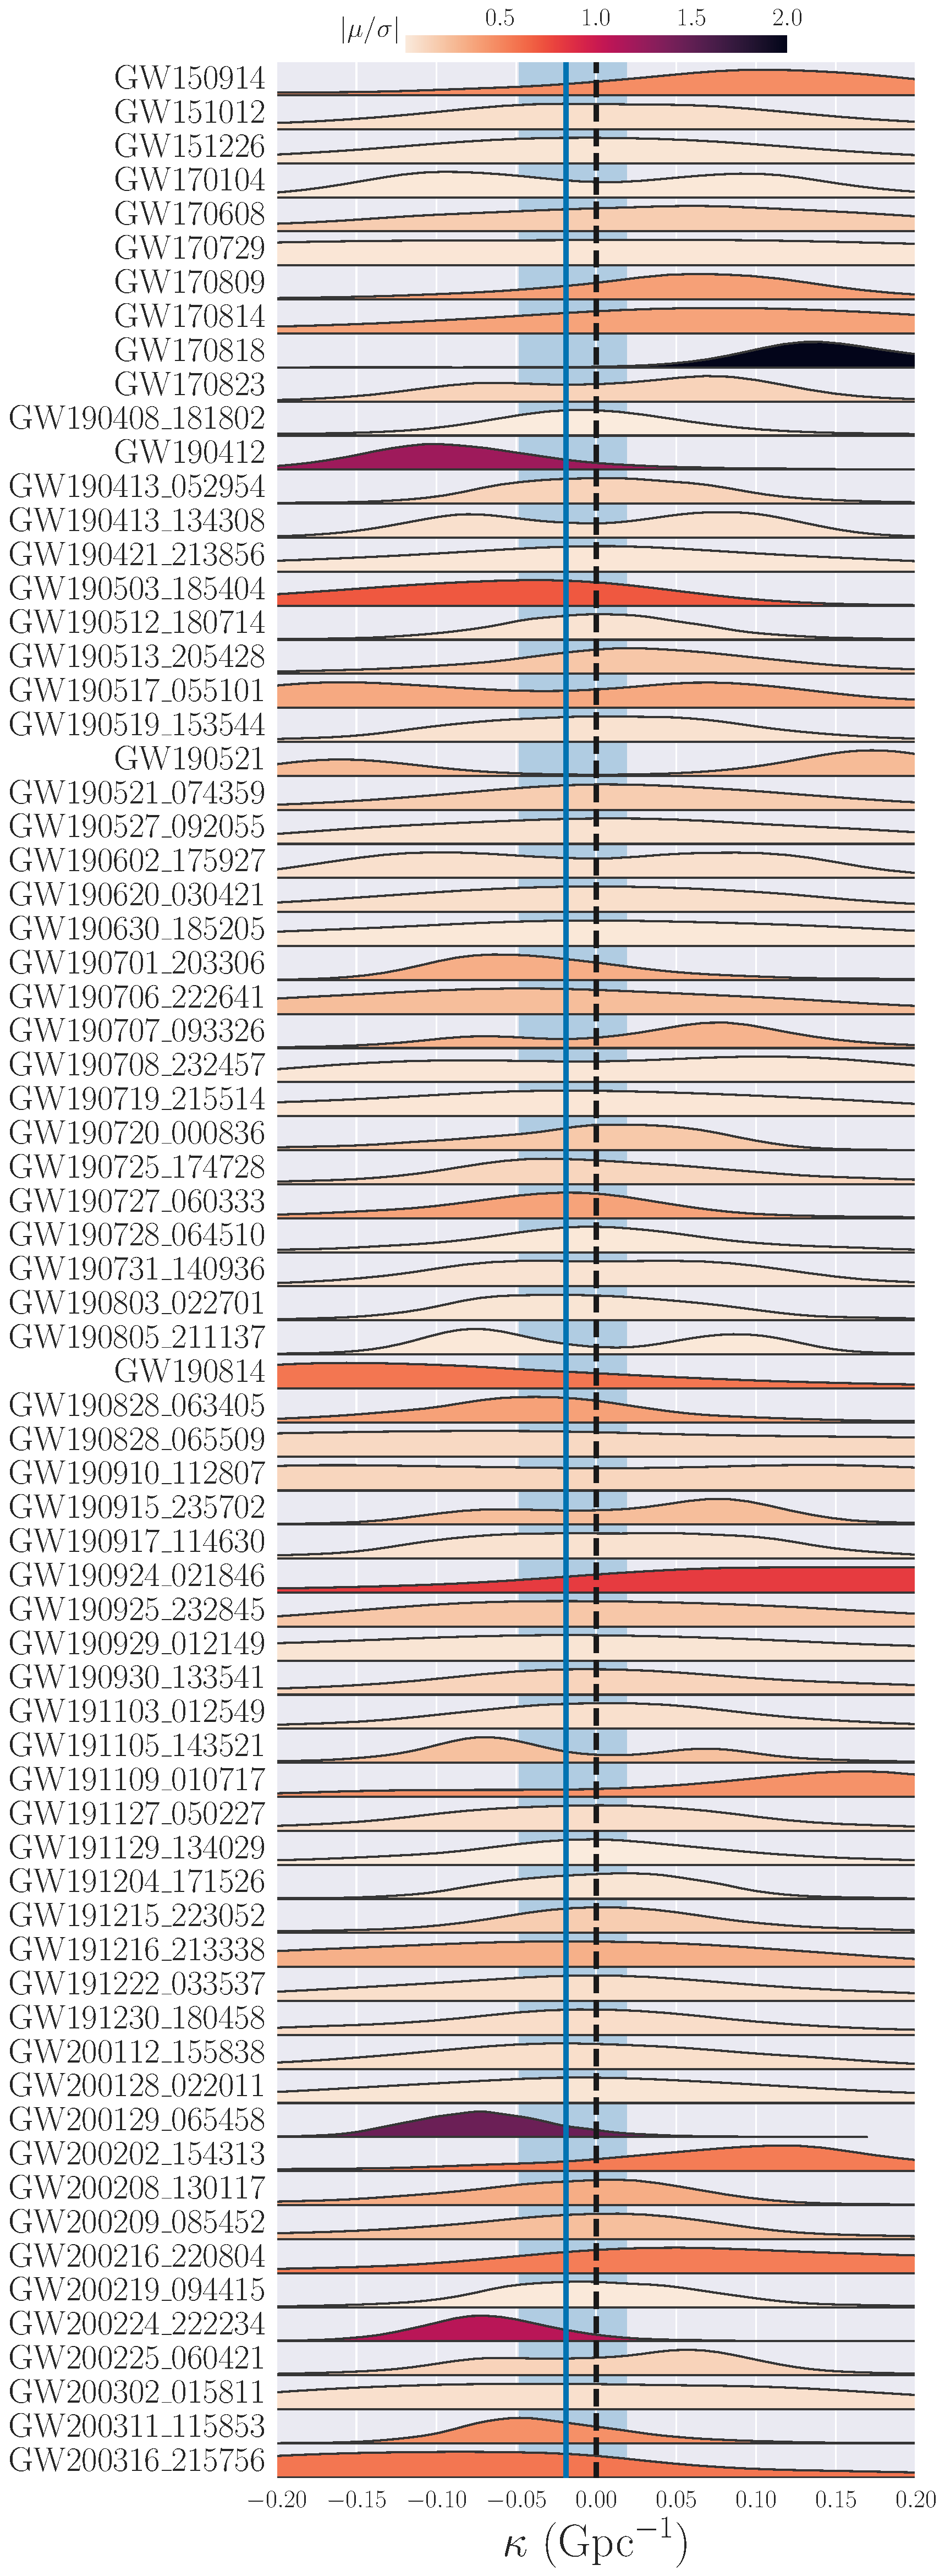
\includegraphics[width=\textwidth]{figures/violin_kappa.pdf}
    \caption{
        The violin plot shows the posterior of $\kappa$ for 69 events in this study.
        Each violin represents a different event.
        The color of the violins represents the quotient of the median and standard deviation of the posterior.
        The orange horizontal solid line represents the median of $\kappa$, and the orange dashed lines enclose the $90\%$ confidence interval.
        The yellow horizontal solid line represents $\kappa=0$.
    }
    \label{fig:violin_kappa}
\end{figure*}

\subsection{Bayesian hierarchical modeling}
% Corner plot of the mean and standard deviation of kappa
The posterior of $\mu$ and $\sigma$ are shown in figure \ref{fig:corner_Gaussian}.
The median of $\mu$ within $90\%$ confidence interval is \variable{output/mu_median.txt}.
The median of $\sigma$ within $90\%$ confidence interval is \variable{output/sigma_median.txt}.
The posterior of $\mu$ is concentrated around $0$, which means the population constraint on $\kappa$ is consistent with GR.

\begin{figure}[h]
    \script{corner_Gaussian.py}
    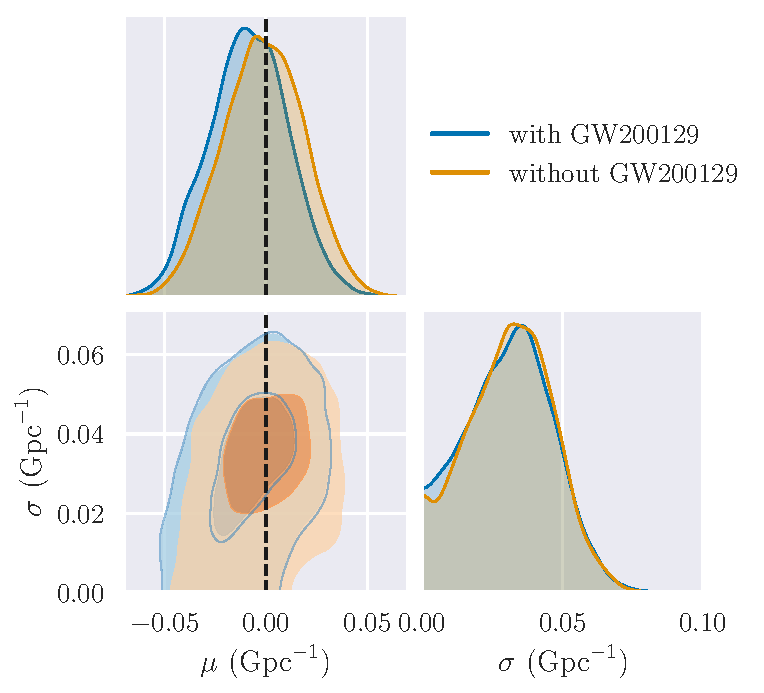
\includegraphics[width=\columnwidth]{figures/corner_Gaussian.pdf}
    \caption{
        The posterior of $\mu$ and $\sigma$ of the population distribution of $\kappa$.
        2D contour plot shows $39.35\%$ and $90\%$ confidence level.
        The orange line represents the median of $\mu$ and $\sigma$.
        The plot shows that the population constraint on $\kappa$ is consistent with GR.
    }
    \label{fig:corner_Gaussian}
\end{figure}

\subsection{Constaint on $\kappa$}
% Constraint on $\kappa$
In figure \ref{fig:posterior_kappa}, we show both the restricted posterior of $\kappa$ and the generic posterior of $\kappa$.
The restricted posterior of $\kappa$ is calculated by equation \ref{eq:restricted_posterior} with the assumption that $\kappa$ is a single value constant.
The generic posterior of $\kappa$ is calculated by equation \ref{eq:generic_posterior} with the assumption that $\kappa$ is a true value drawn from a Gaussian distribution.
The median of the restricted posterior of $\kappa$ within $90\%$ confidence interval is \variable{output/restricted_kappa_median.txt}.
The median of the generic posterior of $\kappa$ within $90\%$ confidence interval is \variable{output/generic_kappa_median.txt}.
Note that the result is consistent with GR when $\kappa=0$.

\begin{figure}[h]
    \script{posterior_kappa.py}
    \includegraphics[width=\columnwidth]{figures/posterior_kappa.pdf}
    \caption{
        The generic and restricted posterior of $\kappa$.
        The orange solid line shows the restricted posterior of $\kappa$, and the orange dashed lines enclose the $90\%$ confidence interval.
        The blue solid line shows the generic posterior of $\kappa$, and the blue dashed lines enclose the $90\%$ confidence interval.
        The pink vertical solid line represents $\kappa=0$.
    }
    \label{fig:posterior_kappa}
\end{figure}

% Case study
% Case: GW170818

% Case: GW150914 (example of broken degeneracy)
\subsection{Result on GW150914}
In this study, we included frequency dependence of birefringence, which would affect the posterior of $\kappa$ obtained from PE.
Consider GW150914, the first GW detected by LIGO, as an example.
In figure \ref{fig:corner_GW150914}, we show the posteriors of the parameters of GW150914.
With the frequency-independent birefringence model, the posteriors for $\cos\iota$ look different from the posteriors assuming GR.
This is because, for a nonprecessing system, there is a degeneracy between $\kappa$ and $\iota$ if the frequency dependence is not included.
% explain the kappa gap

On the other hand, with the frequency-dependent birefringence model, the posterior looks similar to the GR posterior.
This is because the frequency dependence broke the degeneracy, as the effect of birefringence will differ from the effect of changing $\iota$.
In this case, the most probable value of $\kappa$ is close to $0$, which means the birefringence is weak or absent.
Therefore, the PE result with frequency dependence is consistent with GR.

\begin{figure}[h]
    \script{corner_GW150914.py}
    \includegraphics[width=\columnwidth]{figures/corner_GW150914.pdf}
    \caption{
        The posterior of $\kappa$, luminosity distance $d_L$ and $\cos{\iota}$ for GW150914.
        Colors in the plot represent the PE result with GR done by LVK without cosmological reweighing \citep{GWTC-2.1, GWTC-3}, the PE results done by us with both frequency independent and dependent birefringence respectively.
        2D contour plot shows $39.35\%$ and $90\%$ confidence level.
        Note that there is no posterior of $\kappa$ for the PE result from LVK, as the LVK PE is based on GR, which does not suggest GW amplitude birefringence.
        This plot shows that frequency-independent birefringence creates a degeneracy between $\kappa$ and $\iota$, while frequency-dependent birefringence can break it.
    }
    \label{fig:corner_GW150914}
\end{figure}

% Case: GW190521 (massive BBH)
\subsection{Result on GW190521}
Even with the frequency-dependent birefringence model, some events still have a bimodal $\kappa$ distribution.
Consider GW190521, the most massive binary black hole merger in the events we included.
The degeneracy between $\kappa$ and $\iota$ cannot be broken by the frequency-dependent birefringence model, as shown in figure \ref{fig:corner_GW190521}.
The reason could be this GW event's frequency range is too narrow to break the degeneracy.
The effect of birefringence at different frequencies within the range is similar, so the degeneracy cannot be broken.
Therefore, the narrow frequency range can be a possible reason why the $\kappa$ distribution of GW190521 is bimodal.

\begin{figure}[h]
    \script{corner_GW190521.py}
    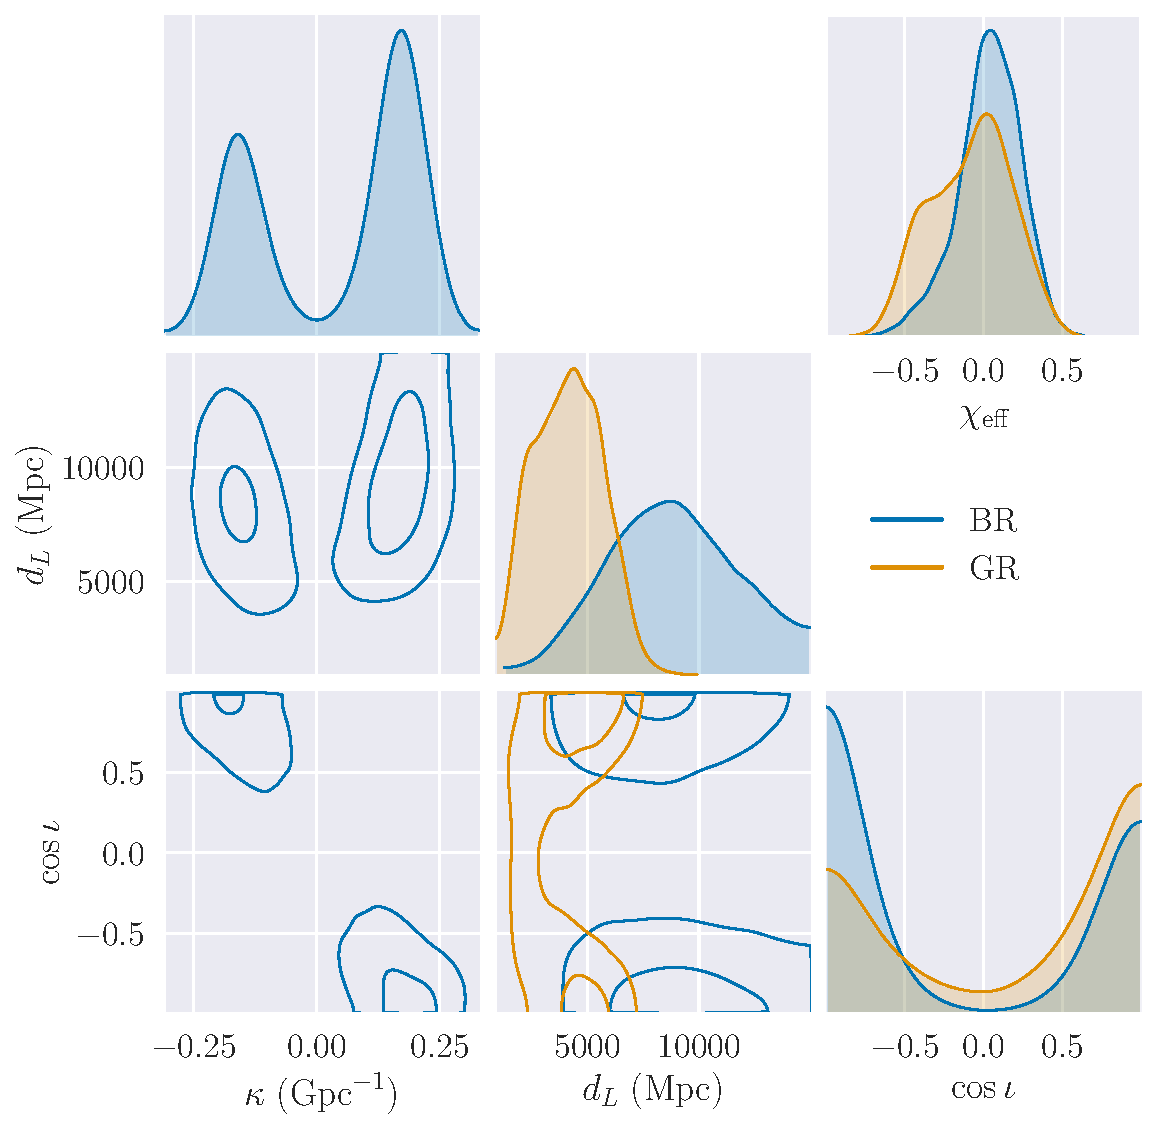
\includegraphics[width=\columnwidth]{figures/corner_GW190521.pdf}
    \caption{
        The posterior of $\kappa$, luminosity distance $d_L$ and $\cos{\iota}$ for GW190521.
        Colors in the plot are the PE result with GR done by LVK without cosmological reweighing \citep{GWTC-2.1, GWTC-3} and the PE result done by us with the frequency-dependent birefringence.
        2D contour plot shows $39.35\%$ and $90\%$ confidence level.
        This plot shows that frequency-dependent birefringence cannot break the degeneracy between $\kappa$ and $\iota$.
    }
    \label{fig:corner_GW190521}
\end{figure}

% Case: GW200129 (glitch in Virgo data)
\subsection{Exclusion of GW200129}
\label{sec:GW200129}
The reason for the exclusion is that past research suggests a potential glitch in GW200129 Virgo data. \citep{GW200129_glitch}
We perform three sets of PE to check if the glitch would affect the population posterior of $\kappa$.
We pick only two out of three detector data in each set to perform PE.
The two sets of PE results with Virgo data return a $\kappa$ posterior that strongly suggests a negative $\kappa$.
Further investigation is needed to understand the glitch.
Thus, we did not include this event in our analysis.
% show result included and excluded

% Case: GW190720 (failed PE)
\subsection{Exclusion of GW190720}
\label{sec:GW190720}
For GW190720, we could not perform PE with Bilby successfully.
In LVK PE papers \citep{GWTC-2.1, GWTC-3}, the PE of some events was performed with LALInference \citep{lalsuite} instead of Bilby.
GW190720 was one of them.
We successfully migrated the LALInference configuration to Bilby for most of these events and recovered similar PE results, except for GW190720.
Bilby could not evaluate the likelihood function on Virgo data.
As a result, we excluded this event from our analysis.

\section{Discussion}
\label{sec:Discussion}

% Comparison with previous studies
\subsection{Comparison with Previous Studies}
\citet{Okounkova_2022} gave a constraint on GW amplitude birefringence by performing statistical analysis on GWTC-2.
We convert the constraint to the same format as ours to make a comparison.
They were able to constrain $\kappa$ to be $|\kappa| \lesssim 0.74$ at $1 \sigma$.
We obtained a tighter constraint on $\kappa$ with $|\kappa| \lesssim 0.04$ at $1 \sigma$.
Our result is an order of magnitude improvement in constraining $\kappa$.
The main reason is that we have more events from GWTC-3 than GWTC-2.

% Future work
\subsection{Future Work}
% BNS
Future work is to perform PE on binary neutron star mergers, such as GW170817.
The frequency range of the signal is much wider compared to the binary black hole mergers.
Thus, the difference in the effect of birefringence at different frequencies within the range can be more significant.
The PE on binary neutron star mergers can allow us to further constrain the birefringence effect and the beyond-GR theories that predict it.
However, performing PE on binary neutron star mergers requires much more computational resources.
Therefore, we may need to wait for future PE methods and tools to further our work.

% More observations with higher SNR
Another future work is to apply the same method to more GW events and events with a higher signal-to-noise ratio (SNR).
LVK will release more events with higher SNR in the future.
Using data with higher SNR allows us to obtain more precise PE results and constrain the birefringence effect more precisely.
And using data from more events will allow us to calculate a more constrained population posterior of $\kappa$.

\section{Acknowledgements}
\label{sec:Acknowledgements}
M.~I., K.~W.~K.~W.~, and W.~M.~F.~ are funded by the Center for Computational Astrophysics at the Flatiron Institute.
The Flatiron Institute provided the computational resources used in this work.

This research has made use of data or software obtained from the Gravitational Wave Open Science Center (gwosc.org), a service of LIGO Laboratory, the LIGO Scientific Collaboration, the Virgo Collaboration, and KAGRA.
LIGO Laboratory and Advanced LIGO are funded by the United States National Science Foundation (NSF) as well as the Science and Technology Facilities Council (STFC) of the United Kingdom, the Max-Planck-Society (MPS), and the State of Niedersachsen/Germany for support of the construction of Advanced LIGO and construction and operation of the GEO600 detector.
Additional support for Advanced LIGO was provided by the Australian Research Council.
Virgo is funded, through the European Gravitational Observatory (EGO), by the French Centre National de Recherche Scientifique (CNRS), the Italian Istituto Nazionale di Fisica Nucleare (INFN) and the Dutch Nikhef, with contributions by institutions from Belgium, Germany, Greece, Hungary, Ireland, Japan, Monaco, Poland, Portugal, Spain.
KAGRA is supported by Ministry of Education, Culture, Sports, Science and Technology (MEXT), Japan Society for the Promotion of Science (JSPS) in Japan; National Research Foundation (NRF) and Ministry of Science and ICT (MSIT) in Korea; Academia Sinica (AS) and National Science and Technology Council (NSTC) in Taiwan.

\pagebreak
\bibliography{bib}

\end{document}
